\documentclass[usenames, xcolor=dvipsnames]{beamer}
%% \documentclass[professionalfonts, xcolor=table, handout]{beamer}
%% \usepackage{pgfpages}
%% \pgfpagesuselayout{4 on 1}[a4paper,border shrink=5mm, landscape]
\usepackage{fontspec}
\usepackage{amsmath,amssymb}
\usepackage{pifont}% http://ctan.org/pkg/pifont
\usepackage{tikz}
\usetikzlibrary{positioning, matrix, arrows.meta, shapes.geometric, calc,
  decorations.pathmorphing, decorations.pathreplacing, fit, shapes.multipart}
\usepackage{mathabx}
\usepackage{mathtools}
\usepackage{mathpartir}
\usepackage{fancyvrb}
\usepackage{stmaryrd}
\usepackage[absolute,overlay]{textpos}
\definecolor{lightg}{RGB}{217,232,225}
\definecolor{darkg}{RGB}{6,81,42}
\definecolor{myred}{rgb}{0.89, 0.45, 0.36}
\colorlet{mypink}{myred!50!white}
\colorlet{mymaroon}{red!70!black}

\defaultfontfeatures{Mapping=tex-text,Scale=MatchLowercase}
% \setmainfont{Libertinus Serif}
% \setsansfont{Libertinus Sans}
% \setmonofont{Menlo Regular}
\usetheme{Madrid}
\useoutertheme{infolines} % Alternatively: miniframes, infolines, split
\useinnertheme{circles}

% \setbeamertemplate{enumerate item}[default]
\usecolortheme[named=myred]{structure}
% \usecolortheme{spruce}
\usefonttheme{serif}
\setbeamerfont*{frametitle}{series=\bfseries}
\setbeamercolor{alerted text}{fg=mymaroon}
\setbeamertemplate{navigation symbols}{}
\setbeamercolor{emphC}{fg=myred}
% \setbeamercolor{block title}{bg = darkg, fg=white!80}
% \setbeamercolor{block body}{bg = lightg, fg=black}
\setbeamercolor{itemize item}{fg=black}
\setbeamercolor{description item}{fg=myred}

\newcommand{\scon}{\mathbin{\ast}}
\newcommand{\ocon}{%
  \mathbin{\mbox{$\mathrlap{\cup}\hspace*{.15em}
      \raisebox{.01em}[0ex][0ex]{$\scon$}$\hspace*{.07em}}}}
\newcommand{\medocon}{
  \raisebox{-0.3ex}{\resizebox{0.63em}{!}{$\scon$}} \hspace{-2.4ex} \bigcup}
\newcommand{\wand}{%
 \mathrel{\mbox{$\hspace*{-0.03em}\mathord{-}\hspace*{-0.66em}
  \mathord{-}\hspace*{-0.36em}\mathord{\scon}$\hspace*{-0.005em}}}}
\newcommand{\defeq}{\mathbin{\overset{\mathrm{def}}{=}}}
\newcommand{\emphd}[1]{{\bfseries #1}}
\newcommand{\emphr}[2]{\alert<#1>{#2}}
\newcommand{\bracket}[1]{[#1]}
\newcommand{\hide}[1]{}
\makeatletter\let\frametextheight\beamer@frametextheight\makeatother
\newcommand\credit[1]{%
  \begin{textblock*}{\paperwidth}(0pt,\textheight)
    \raggedleft #1\hspace{.5em}
\end{textblock*}}
\newcommand{\pguards}[1]{\llbracket #1 \rrbracket}
\newcommand{\xmark}{\ding{55}}%
\newcommand{\cmark}{\ding{51}}%

\title[Verified GC for Gallina]{A Verified Garbage Collector for Gallina}
\author[Wang, Mohan, Hobor]{\hspace{-0.5em}Shengyi Wang, 
\underline{Anshuman Mohan}, Aquinas Hobor}
\institute[NUS]{\includegraphics[height=0.12\textwidth]{NUS_logo_full-horizontal.jpg}}
\date[APLAS NIER 2019]{APLAS NIER \\ \today}

\begin{document}
\begin{frame}
  \titlepage
\end{frame}

\section{Introduction}

\begin{frame}{Broad Problem}
Verify \alert{graph-manipulating} programs
\\ \hspace{1em}written in \alert{executable C}
\\ \hspace{2em}with \alert{machine-checked} correctness proofs
\bigskip
\uncover<2->{\flushright{Ubiquitous in critical areas}}
\end{frame}

\begin{frame}{Broad Solution}
\includegraphics[scale=0.09]{vst_logo}
\hspace{2em} \includegraphics[scale=0.12]{compcert_logo}
\hspace{2em} \includegraphics[scale=0.2]{paper_screen}

\bigskip
VST + CompCert + 40000 \textsc{loc} library

\pause
\bigskip
Powerful enough to verify \alert{executable code}
\\\hspace{1em}against \alert{realistic specifications}
\\\hspace{2em}expressed with \alert{mathematical graphs}

\pause 
\bigskip
\flushright [{\footnotesize Wang \emph{et. al.}}, \textsc{pacmpl oopsla} {\footnotesize 2019}]
\end{frame}

\begin{frame}{This Talk}
\includegraphics[scale=0.02]{certicoq_logo} 
\hspace{2em} \includegraphics[scale=0.12]{compcert_logo}

\bigskip
Gallina \alert<2->{$\leadsto$} CompCert C $\leadsto$ Assembly

\bigskip \pause \pause
Gallina assumes \alert{infinite} memory
\\\hspace{1em} but CompCert C has a \alert{finite} heap

\bigskip
\pause Solution: garbage collect the CompCert C code

\pause
\flushright{\alert{New problem: verify the garbage collector}}
\end{frame}

\section{Specification}

\begin{frame}{Garbage Collection: an Introduction}
\uncover<1->{GC has jurisdiction over the heap}
\uncover<3->{\\\hspace{1em} Mutator $\texttt{malloc}$s in special subheap}
\uncover<4->{\\\hspace{2em} If subheap is full} 
\uncover<5->{\alert{call GC}}
\uncover<6->{and try again}

\bigskip

\begin{center}
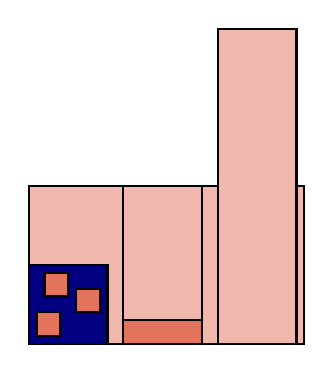
\begin{tikzpicture}
\uncover<1>{\draw [fill=mypink, thick] 
  (0,0) -- (3.5,0) -- (3.5,2) -- (0,2) -- cycle;}
\uncover<2->{\draw [fill=mypink, thick] 
  (0,0) -- (1,0) -- (1,1) -- (0,1) -- cycle;
            \draw [fill=mypink, thick] 
  (1.2,0) -- (2.2,0) -- (2.2,2) -- (1.2,2) -- cycle;
            \draw [fill=mypink, thick] 
  (2.4,0) -- (3.4,0) -- (3.4,4) -- (2.4,4) -- cycle;}
\uncover<3,6>{\draw [fill=myred, thick]
  (0.1,0.1) -- (0.4,0.1) -- (0.4,0.4) -- (0.1,0.4) -- cycle;}
\uncover<4>{\draw [fill=NavyBlue, thick]
  (0,0) -- (1,0) -- (1,1) -- (0,1) -- cycle;
            \draw [fill=myred, thick]
  (0.1,0.1) -- (0.4,0.1) -- (0.4,0.4) -- (0.1,0.4) -- cycle;
            \draw [fill=myred, thick]
  (0.6,0.4) -- (0.9,0.4) -- (0.9,0.7) -- (0.6,0.7) -- cycle;
            \draw [fill=myred, thick]
  (0.2,0.6) -- (0.5,0.6) -- (0.5,0.9) -- (0.2,0.9) -- cycle;
  }
\uncover<5->{\draw [fill=myred, thick]
  (1.2,0) -- (2.2,0) -- (2.2,0.3) -- (1.2,0.3) -- cycle;}
\end{tikzpicture}
\end{center}
\end{frame}

\begin{frame}{Intuitive Specification}
\emph{Primum non nocere}: first, do no harm

\bigskip

\begin{center}
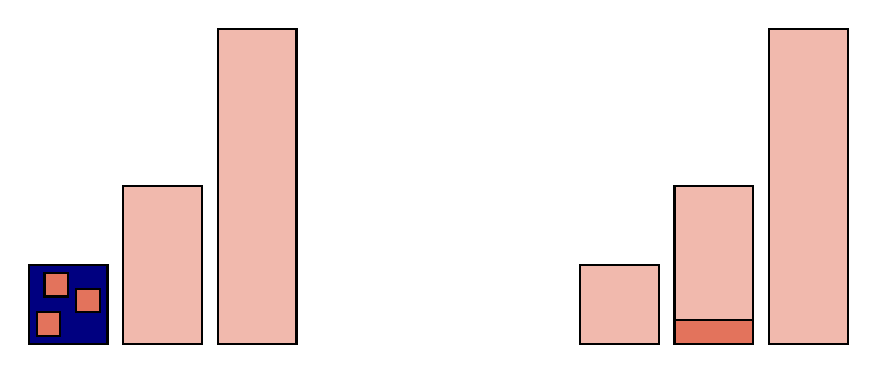
\begin{tikzpicture}
\uncover<2->{
            \draw [fill=NavyBlue, thick]
  (0,0) -- (1,0) -- (1,1) -- (0,1) -- cycle;
            \draw [fill=myred, thick]
  (0.1,0.1) -- (0.4,0.1) -- (0.4,0.4) -- (0.1,0.4) -- cycle;
            \draw [fill=myred, thick]
  (0.6,0.4) -- (0.9,0.4) -- (0.9,0.7) -- (0.6,0.7) -- cycle;
            \draw [fill=myred, thick]
  (0.2,0.6) -- (0.5,0.6) -- (0.5,0.9) -- (0.2,0.9) -- cycle;
            \draw [fill=mypink, thick ] 
  (1.2,0) -- (2.2,0) -- (2.2,2) -- (1.2,2) -- cycle;
            \draw [fill=mypink, thick ] 
  (2.4,0) -- (3.4,0) -- (3.4,4) -- (2.4,4) -- cycle;}
\tikzset{shift={(7,0)}}
  \uncover<3->{
            \draw [fill=mypink, thick ]
  (0,0) -- (1,0) -- (1,1) -- (0,1) -- cycle;
            \draw [fill=mypink, thick ] 
  (1.2,0) -- (2.2,0) -- (2.2,2) -- (1.2,2) -- cycle;
            \draw [fill=mypink, thick ] 
  (2.4,0) -- (3.4,0) -- (3.4,4) -- (2.4,4) -- cycle;
  \draw [fill=myred, thick]
  (1.2,0) -- (2.2,0) -- (2.2,0.3) -- (1.2,0.3) -- cycle;}
  \end{tikzpicture}
\end{center}

\uncover<4>{\vspace{-6em}\hspace{5.8cm}\Huge $\cong$}
\end{frame}


\section{Our Garbage Collector}

\begin{frame}{Our Garbage Collector}
  \begin{itemize}
  \item 12 generations, doubling in size
  \item Functional mutator: no back pointers
  \pause
  \item Cheney's mark-and-copy collects gen to next
  \item Potentially triggers cascade of pairwise collections
  \pause
  \item Three key functions: 
  \\\hspace{1em}\texttt{forward} copies individual objects
  \\\hspace{1em}\texttt{do\_scan} repairs copied objects
  \\\hspace{1em}\texttt{forward\_roots} kick-starts the collection
  \end{itemize}
\end{frame}

\newcommand{\ws}[1]{\color{white}{\scriptsize #1}}

\begin{frame}[fragile]{Overview of Operation'}
  \begin{center}
  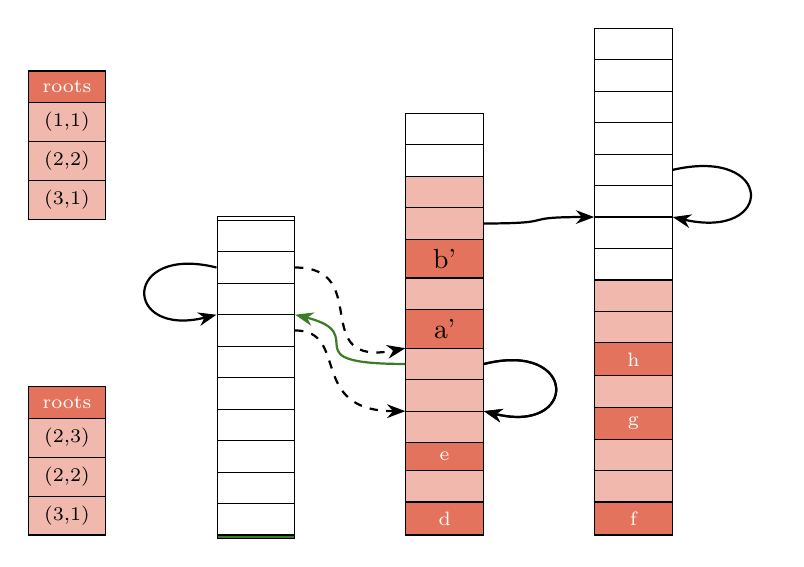
\begin{tikzpicture}[heap/.style={rectangle split, rectangle split parts=#1, draw,
        minimum width=28pt}, node distance=1.4cm, ->/.style={-Stealth, thick}]
    \node<1> [heap=10, rectangle split part fill={white, white, white, mypink, myred, mypink, mypink, myred, mypink, myred}]
    (gen 0) {\nodepart{ten}\ws{a}
            \nodepart{eight}\ws{b}
            \nodepart{five}\ws{c}};
    \node<2> [heap=10, rectangle split part fill={white, white, white, mypink, myred, mypink, mypink, myred, mypink, OliveGreen}]
    (gen 0) {\nodepart{ten}\ws{a}
            \nodepart{eight}\ws{b}
            \nodepart{five}\ws{c}};
    \node<3> [heap=10, rectangle split part fill={white, white, white, mypink, myred, mypink, mypink, OliveGreen, mypink, OliveGreen}]
    (gen 0) {\nodepart{ten}\ws{a}
            \nodepart{eight}\ws{b}
            \nodepart{five}\ws{c}};
    \node<4> [heap=10, rectangle split part fill={white, white, white, mypink, NavyBlue, mypink, mypink, myred, mypink, OliveGreen}]
    (gen 0) {\nodepart{ten}\ws{a}
            \nodepart{eight}\ws{b}
            \nodepart{five}\ws{c}};
    \node<5> [heap=10, rectangle split part fill={white}] (gen 0) {};

    \node<1>[heap=13, right = of gen 0.south east, anchor=south west,
      rectangle split part fill={white, white, white, white, white, white, white, mypink, mypink, mypink, myred, mypink, myred}]
        (gen 1) {\nodepart{thirteen}\color{white}{\scriptsize d}
                 \nodepart{eleven}\color{white}{\scriptsize e}};
    \node<2>[heap=13, right = of gen 0.south east, anchor=south west,
      rectangle split part fill={white, white, white, white, white, mypink, myred, mypink, mypink, mypink, myred, mypink, myred}]
        (gen 1) {\nodepart{thirteen}\color{white}{\scriptsize d}
                 \nodepart{eleven}\color{white}{\scriptsize e}
                 \nodepart{seven}\ws{a'}};
    \node<3->[heap=13, right = of gen 0.south east, anchor=south west,
      rectangle split part fill={white, white, mypink, mypink, myred, mypink, myred, mypink, mypink, mypink, myred, mypink, myred}]
        (gen 1) {\nodepart{thirteen}\color{white}{\scriptsize d}
                 \nodepart{eleven}\color{white}{\scriptsize e}
                 \nodepart{seven}\ws{a'}
                 \nodepart{five}\ws{b'}};

    \node<1-> [heap=16, right = of gen 1.south east, anchor=south west,
      rectangle split part fill={white, white, white, white, white, white, white, white, mypink, mypink, myred, mypink, myred, mypink, mypink, myred}]
    (gen 2) {\nodepart{sixteen}\color{white}{\scriptsize f}\nodepart{thirteen}\color{white}{\scriptsize g}\nodepart{eleven}\color{white}{\scriptsize h}};
        
    \node<1> [heap=4, left = of gen 0.north west, anchor=south east,
      rectangle split part fill={myred, mypink, mypink, mypink}] (roots) {\color{white}\scriptsize roots\nodepart{two}{\scriptsize (1,1)}\nodepart{three}{\scriptsize (2,2)}\nodepart{four}{\scriptsize (3,1)}};
    \node<2-> [heap=4, left = of gen 0.south west, anchor=south east,
      rectangle split part fill={myred, mypink, mypink, mypink}] (roots) {\color{white}\scriptsize roots\nodepart{two}{\scriptsize (2,3)}\nodepart{three}{\scriptsize (2,2)}\nodepart{four}{\scriptsize (3,1)}};

    \draw<4->[->] (gen 1.eight east)..controls +(1.2, 0.3) and +(1.2, -0.3)..
    (gen 1.nine split east);
    \draw[->] (gen 2.five east)..controls +(1.3, 0.3) and +(1.3, -0.3)..
    (gen 2.six split east);
    % \draw[->] (gen 2.two east)..controls +(1, 0.3) and +(1, -0.3)..
    % (gen 2.four split east);
    \draw[->] (gen 1.four east)..controls +(1, 0) and +(-1, 0)..
    (gen 2.six split west);
    \draw<1>[->] (gen 0.two west)..controls +(-1.2, 0.3) and +(-1.2, -0.3)..
    (gen 0.three split west);
    \draw<2,3,4>[->,dashed] (gen 0.two east)..controls +(1, 0) and +(-1.25, -0.25)..
    (gen 1.seven split west);
    \draw<2,3>[->,OliveGreen] (gen 1.eight west)..controls +(-1.5, 0) and +(1, -0.25)..
    (gen 0.three split east);
    \draw<3,4>[->,dashed] (gen 0.four east)..controls +(0.7, 0) and +(-1.25, 0)..
    (gen 1.nine split west);
    \draw<4->[->] (gen 1.eight east)..controls +(1.2, 0.3) and +(1.2, -0.3)..
    (gen 1.nine split east);

  \end{tikzpicture}
  \end{center}

\uncover<2->{\texttt{forward} \cmark}
\uncover<4->{\hspace{2em}\texttt{do\_scan} \cmark}
\uncover<5->{\hspace{2em}\texttt{do\_gen} \cmark}
\end{frame}

% \begin{frame}[fragile]{Overview of Operation}
%   \begin{center}
%   \begin{tikzpicture}[heap/.style={rectangle split, rectangle split parts=#1, draw,
%         minimum width=32pt}, node distance=1.7cm, ->/.style={-Stealth, thick}]
%     \node<1> [heap=10, rectangle split part fill={myred, mypink,
%         myred, mypink, mypink, myred, mypink, white}]
%     (gen 0) {\color{white}{\scriptsize a}\nodepart{three}\color{white}{\scriptsize b}\nodepart{six}\color{white}{\scriptsize c}};
%     \node<2> [heap=10, rectangle split part fill={OliveGreen, mypink,
%         myred, mypink, mypink, myred, mypink, white}]
%     (gen 0) {\color{white}{\scriptsize a}\nodepart{three}\color{white}{\scriptsize b}\nodepart{six}\color{white}{\scriptsize c}};
%     \node<3> [heap=10, rectangle split part fill={OliveGreen, mypink,
%         OliveGreen, mypink, mypink, myred, mypink, white}]
%     (gen 0) {\color{white}{\scriptsize a}\nodepart{three}\color{white}{\scriptsize b}\nodepart{six}\color{white}{\scriptsize c}};
%     \node<4> [heap=10, rectangle split part fill={OliveGreen, mypink,
%         OliveGreen, mypink, mypink, NavyBlue, mypink, white}]
%     (gen 0) {\color{white}{\scriptsize a}\nodepart{three}\color{white}{\scriptsize b}\nodepart{six}\color{white}{\scriptsize c}};
%     \node<5> [heap=10, rectangle split part fill={white}] (gen 0) {};

%     \node<1>[heap=13, right = of gen 0.north east, anchor=north west,
%       rectangle split part fill={myred, mypink, myred,
%         mypink, mypink, mypink, white}]
%         (gen 1) {\color{white}{\scriptsize d}\nodepart{three}\color{white}{\scriptsize e}};
%     \node<2>[heap=13, right = of gen 0.north east, anchor=north west,
%       rectangle split part fill={myred, mypink, myred,
%         mypink, mypink, mypink, myred, mypink, white}]
%         (gen 1) {\color{white}{\scriptsize d}\nodepart{three}\color{white}{\scriptsize e}\nodepart{seven}\color{white}{\scriptsize a}};
%     \node<3>[heap=13, right = of gen 0.north east, anchor=north west,
%       rectangle split part fill={myred, mypink, myred,
%         mypink, mypink, mypink, myred, mypink, myred, mypink, mypink,
%         white}] (gen 1)
%         {\color{white}{\scriptsize d}\nodepart{three}\color{white}{\scriptsize e}\nodepart{seven}\color{white}{\scriptsize a}\nodepart{nine}\color{white}{\scriptsize b}};
%     \node<4>[heap=13, right = of gen 0.north east, anchor=north west,
%       rectangle split part fill={myred, mypink, myred,
%         mypink, mypink, mypink, myred, mypink, myred, mypink, mypink,
%         white}]
%         (gen 1) {\color{white}{\scriptsize d}\nodepart{three}\color{white}{\scriptsize e}\nodepart{seven}\color{white}{\scriptsize a}\nodepart{nine}\color{white}{\scriptsize b}};
%     \node<5>[heap=13, right = of gen 0.north east, anchor=north west,
%       rectangle split part fill={myred, mypink, myred,
%         mypink, mypink, mypink, myred, mypink, myred, mypink, mypink,
%         white}]
%         (gen 1) {\color{white}{\scriptsize d}\nodepart{three}\color{white}{\scriptsize e}\nodepart{seven}\color{white}{\scriptsize a}\nodepart{nine}\color{white}{\scriptsize b}};

%     \node<1-> [heap=16, right = of gen 1.north east, anchor=north west,
%       rectangle split part fill={myred, mypink, mypink, myred,
%         mypink, myred, mypink, mypink, white}]
%     (gen 2) {\color{white}{\scriptsize f}\nodepart{four}\color{white}{\scriptsize g}\nodepart{six}\color{white}{\scriptsize h}};
        
%     \node<1> [heap=4, left = of gen 0.north west, anchor=north east,
%       rectangle split part fill={myred, mypink, mypink, mypink}] (roots) {\color{white}\scriptsize roots\nodepart{two}{\scriptsize (1,1)}\nodepart{three}{\scriptsize (2,2)}\nodepart{four}{\scriptsize (3,1)}};
%     \node<2-> [heap=4, left = of gen 0.north west, anchor=north east,
%       rectangle split part fill={myred, mypink, mypink, mypink}] (roots) {\color{white}\scriptsize roots\nodepart{two}{\scriptsize (2,3)}\nodepart{three}{\scriptsize (2,2)}\nodepart{four}{\scriptsize (3,1)}};

%     \draw<4->[->] (gen 1.eight east)..controls +(1.2, 0.3) and +(1.2, -0.3)..
%     (gen 1.nine split east);
%     \draw[->] (gen 2.five east)..controls +(1.3, 0.3) and +(1.3, -0.3)..
%     (gen 2.six split east);
%     % \draw[->] (gen 2.two east)..controls +(1, 0.3) and +(1, -0.3)..
%     % (gen 2.four split east);
%     \draw[->] (gen 1.four east)..controls +(1, 0) and +(-1, 0)..
%     (gen 2.six split west);
%     \draw<1>[->] (gen 0.two west)..controls +(-1.2, 0.3) and +(-1.2, -0.3)..
%     (gen 0.three split west);
%     \draw<2,3,4>[->,dashed] (gen 0.two east)..controls +(1, 0) and +(-1.25, -0.25)..
%     (gen 1.seven split west);
%     \draw<2,3>[->,OliveGreen] (gen 1.eight west)..controls +(-1.5, 0) and +(1, -0.25)..
%     (gen 0.three split east);
%     \draw<3,4>[->,dashed] (gen 0.four east)..controls +(0.7, 0) and +(-1.25, 0)..
%     (gen 1.nine split west);
%     \draw<4->[->] (gen 1.eight east)..controls +(1.2, 0.3) and +(1.2, -0.3)..
%     (gen 1.nine split east);

%   \end{tikzpicture}
%   \end{center}

% \uncover<2->{\texttt{forward} \cmark}
% \uncover<4->{\hspace{2em}\texttt{do\_scan} \cmark}
% \uncover<5->{\hspace{2em}\texttt{do\_gen} \cmark}
% \end{frame}

\begin{frame}[fragile]{\emph{Non}-Concerns}
  \begin{center}
  \begin{tikzpicture}[heap/.style={rectangle split, rectangle split parts=#1, draw,
        minimum width=32pt}, node distance=1.7cm, ->/.style={-Stealth, thick}]

    \node<1-> [heap=4, left = of gen 0.north west, anchor=north east,
      rectangle split part fill={myred, mypink, mypink, mypink}] (roots) {\color{white}\scriptsize roots\nodepart{two}{\scriptsize (2,3)}\nodepart{three}{\scriptsize (2,2)}\nodepart{four}{\scriptsize (3,1)}};

    \node<1-> [heap=10, rectangle split part fill={white}] (gen 0) {};


    \node<1->[heap=13, right = of gen 0.north east, anchor=north west,
      rectangle split part fill={NavyBlue, mypink, myred,
        mypink, mypink, mypink, myred, mypink, myred, mypink, mypink,
        white}]
        (gen 1) {\color{white}{\scriptsize d}\nodepart{three}\color{white}{\scriptsize e}\nodepart{seven}\color{white}{\scriptsize a}\nodepart{nine}\color{white}{\scriptsize b}};

    \node<1-> [heap=16, right = of gen 1.north east, anchor=north west,
      rectangle split part fill={myred, mypink, mypink, NavyBlue,
        mypink, myred, mypink, mypink, white}]
    (gen 2) {\color{white}{\scriptsize f}\nodepart{four}\color{white}{\scriptsize g}\nodepart{six}\color{white}{\scriptsize h}};

    \draw<1>[->] (gen 1.eight east)..controls +(1.2, 0.3) and +(1.2, -0.3)..
    (gen 1.nine split east);
    \draw<1>[->] (gen 2.five east)..controls +(1.3, 0.3) and +(1.3, -0.3)..
    (gen 2.six split east);
    % \draw[->] (gen 2.two east)..controls +(1, 0.3) and +(1, -0.3)..
    % (gen 2.four split east);
    \draw<1>[->] (gen 1.four east)..controls +(1, 0) and +(-1, 0)..
    (gen 2.six split west);
    \draw<1>[->] (gen 1.eight east)..controls +(1.2, 0.3) and +(1.2, -0.3)..
    (gen 1.nine split east);
    \draw<2>[->,OliveGreen,dashed] (gen 2.two west)..controls +(-.5, 0) and +(1, -0.25)..
    (gen 1.three split east);
    \draw<2>[->,OliveGreen,dashed] (gen 2.seven west)..controls +(-0.9, -0.3) and +(0, 0)..
    (gen 1.seven split east);
    \draw<2>[->,white] (gen 2.five east)..controls +(1.3, 0.3) and +(1.3, -0.3)..
    (gen 2.six split east);

  \end{tikzpicture}
  \end{center}
\uncover<1->{more garbage? \xmark}
\uncover<2->{\hspace{2em}back pointers? \xmark}
\end{frame}

\begin{frame}[fragile]{Sources of Complexity}
  \begin{center}
  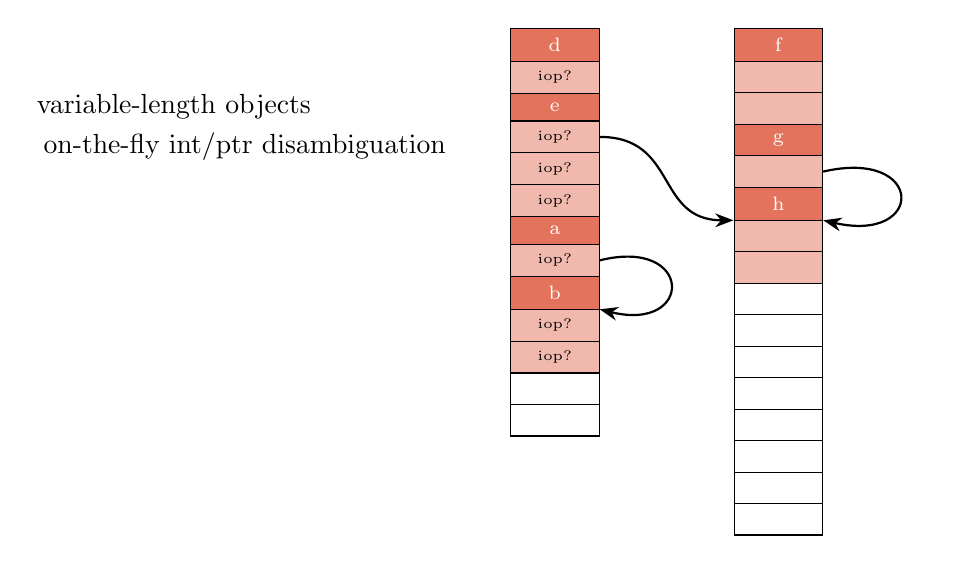
\begin{tikzpicture}[heap/.style={rectangle split, rectangle split parts=#1, draw,
        minimum width=32pt}, heapclear/.style={rectangle split, rectangle split parts=#1,
        minimum width=32pt}, node distance=1.7cm, ->/.style={-Stealth, thick}]
    \node<1-> [heapclear=10, rectangle split part fill={white}] (gen 0) {};

    \node<1>[heap=13, right = of gen 0.north east, anchor=north west,
      rectangle split part fill={myred, mypink, myred,
        mypink, mypink, mypink, myred, mypink, myred, mypink, mypink,
        white}]
        (gen 1) {\color{white}{\scriptsize d}\nodepart{three}\color{white}{\scriptsize e}\nodepart{seven}\color{white}{\scriptsize a}\nodepart{nine}\color{white}{\scriptsize b}};
    \node<2>[heap=13, right = of gen 0.north east, anchor=north west,
      rectangle split part fill={myred, mypink, myred,
        mypink, mypink, mypink, myred, mypink, myred, mypink, mypink,
        white}]
        (gen 1) {\color{white}{\scriptsize d}
        \nodepart{two}{\tiny iop?}
        \nodepart{four}{\tiny iop?}
        \nodepart{five}{\tiny iop?}
        \nodepart{six}{\tiny iop?}
        \nodepart{eight}{\tiny iop?}
        \nodepart{ten}{\tiny iop?}
        \nodepart{eleven}{\tiny iop?}
        \nodepart{nine}\color{white}{\scriptsize b}
        \nodepart{three}\color{white}{\scriptsize e}
        \nodepart{seven}\color{white}{\scriptsize a}
        \nodepart{nine}\color{white}{\scriptsize b}};

    \node<1-> [heap=16, right = of gen 1.north east, anchor=north west,
      rectangle split part fill={myred, mypink, mypink, myred,
        mypink, myred, mypink, mypink, white}]
    (gen 2) {\color{white}{\scriptsize f}\nodepart{four}\color{white}{\scriptsize g}\nodepart{six}\color{white}{\scriptsize h}};
        
    \node<1-> [heapclear=4, left = of gen 0.north west, anchor=north east,
      rectangle split part fill={white}] (roots) {};
    % \node<2-> [heap=4, left = of gen 0.north west, anchor=north east,
    %   rectangle split part fill={myred, mypink, mypink, mypink}] (roots) {\color{white}\scriptsize roots\nodepart{two}{\scriptsize (2,3)}\nodepart{three}{\scriptsize (2,2)}\nodepart{four}{\scriptsize (3,1)}};

    \draw[->] (gen 2.five east)..controls +(1.3, 0.3) and +(1.3, -0.3)..
    (gen 2.six split east);
    \draw[->] (gen 1.four east)..controls +(1, 0) and +(-1, 0)..
    (gen 2.six split west);
    \draw[->,white] (gen 0.two west)..controls +(-1.2, 0.3) and +(-1.2, -0.3)..
    (gen 0.three split west);
    \draw[->] (gen 1.eight east)..controls +(1.2, 0.3) and +(1.2, -0.3)..
    (gen 1.nine split east);
\node<1-> at (-2,1) {variable-length objects};
\node<2> at (-1.1,0.5) {on-the-fly int/ptr disambiguation};
% Which gen is v in? Is_from... gen boundaries?
% Size of gen (for next malloc)
% What is the next free spot?
% malloc fails?
% size of alloc (from mutator) -- can't allocate something larger than the nursery
  \end{tikzpicture}
  \end{center}
\uncover<1>{\color{white}\texttt{forward} \cmark}
\end{frame}


\section{Meat and Potatoes}
\begin{frame}{\texttt{Forward}: a Deep Dive}

\texttt{forward} is \alert{robust} \uncover<5->{and \alert{versatile}}
\pause \\ \hspace{1em} pointer? \uncover<6->{\hspace{6em}called on root set}
\pause \\ \hspace{1em} in \texttt{from} space? \uncover<7->{\hspace{3.15em}called on heap}
\pause \\ \hspace{1em} already forwarded?

\bigskip

\uncover<8->{Specifying \texttt{forward} \emph{functionally} is too hard}
\bigskip
\uncover<9->{\\ \texttt{forward\_relation} explains how \\ 
\hspace{1em}the graph may change because of \texttt{forward}}
\end{frame}

\begin{frame}[fragile]{\texttt{forward\_relation}}
\begin{Verbatim}
Inductive forward_relation (from to : nat) : 
    forward_t -> LGraph -> LGraph -> Prop :=
\end{Verbatim}
\pause
\begin{Verbatim}
| fr_v_not_in : forall (v : VType) (g : LGraph),
    vgeneration v <> from ->
    forward_relation from to (inl (inr v)) g g
\end{Verbatim}
\pause
\begin{Verbatim}
| fr_e_to_fwded : forall (e : EType) (g : LGraph),
    vgeneration (dst g e) = from ->
    raw_mark (vlabel g (dst g e)) = true ->
    let new_g := labeledgraph_gen_dst g e
      (copied_vertex (vlabel g (dst g e))) in
    forward_relation from to (inr e) g new_g
\end{Verbatim}
\end{frame}

\begin{frame}[fragile]{\texttt{forward\_relation}, \emph{cont.}}
\begin{Verbatim}
| fr_e_to_not_fwded_Sn : forall (e : EType) (g g' : LGraph), 
    vgeneration (dst g e) = from ->
    raw_mark (vlabel g (dst g e)) = false -> 
    let new_g :=
      labeledgraph_gen_dst (lgraph_copy1v g (dst g e) to)
      e (copy1v_new_v g to) in forward_loop from to
      (make_fields new_g (copy1v_new_v g to)) new_g g' ->
      forward_relation from to (inr e) g g'
\end{Verbatim} 
\pause
\begin{Verbatim}
  with forward_loop (from to : nat) : 
    list field_t -> LGraph -> LGraph -> Prop :=
| fl_nil : forall (g : LGraph), forward_loop from to  [] g g
| fl_cons : forall (g1 g2 g3 : LGraph) 
                   (f : field_t) (fl : list field_t),
      forward_relation from to  (field2forward f) g1 g2 ->
      forward_loop from to  fl g2 g3 ->
      forward_loop from to  (f :: fl) g1 g3
\end{Verbatim}
\end{frame}

\begin{frame}{Specification}
Similar to \texttt{forward\_relation}, we have
\\ \hspace{1em}\texttt{forward\_roots\_relation}
\\ \hspace{1em}\texttt{do\_scan\_relation}
\\ \hspace{1em}\texttt{do\_generation\_relation}
\\ \hspace{1em}\texttt{garbage\_collect\_relation}
% we specify is operationally

\bigskip

\flushright \pause A composition of these gives us our \alert{isomorphism}
\end{frame}

\begin{frame}{More Meat and Potatoes}

\end{frame}

\section{Findings}

\begin{frame}[fragile]{Bugs in the source C code}
  \begin{itemize}
  \item Cheney implemented too conservatively:\\ 
  \hspace{1em}only part of \texttt{to} space needs to be scanned
  \pause 
  \\ Performance doubled
\pause  \bigskip
\item Overflow in the following calculation:
\begin{verbatim}
int space_size =
     h->spaces[i].limit - h->spaces[i].start;
\end{verbatim}
\pause
Fixed by adjusting nursery size
  \end{itemize}
\end{frame}

\begin{frame}[fragile]{Undefined behavior in C}
 Double-bounded pointer comparisons:
    \begin{Verbatim}
int Is_from(value * lo, value * hi, value * v) {
    return (lo <= v && v < hi); }
    \end{Verbatim}
    
\begin{center}
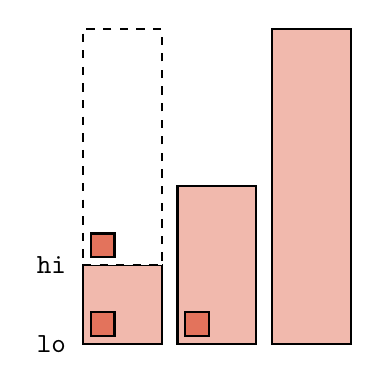
\begin{tikzpicture}
\node at (-0.4,0) {\texttt{lo}};
\node at (-0.4,1) {\texttt{hi}};

% drawing the gens
\draw [fill=mypink, thick] 
  (0,0) -- (1,0) -- (1,1) -- (0,1) -- cycle;
            \draw [fill=mypink, thick] 
  (1.2,0) -- (2.2,0) -- (2.2,2) -- (1.2,2) -- cycle;
            \draw [fill=mypink, thick] 
  (2.4,0) -- (3.4,0) -- (3.4,4) -- (2.4,4) -- cycle;

% drawing the extra malloc portion of from space
\draw<3> [fill=white, dashed, thick] 
  (0,1) -- (1,1) -- (1,4) -- (0,4) -- cycle;

% drawing v in different places
\uncover<2>{\draw [fill=myred, thick]
  (0.1,0.1) -- (0.4,0.1) -- (0.4,0.4) -- (0.1,0.4) -- cycle;}
\uncover<3>{\draw [fill=myred, thick]
  (0.1,1.1) -- (0.4,1.1) -- (0.4,1.4) -- (0.1,1.4) -- cycle;}
\uncover<4->{\draw [fill=myred, thick]
  (1.3,0.1) -- (1.6,0.1) -- (1.6,0.4) -- (1.3,0.4) -- cycle;}
\end{tikzpicture}
\end{center}

\uncover<5>{
Resolved using CompCert's \texttt{extcall\_properties}}
    \end{frame}

\begin{frame}[fragile]{Undefined behavior in C, \emph{cont.}}  
A classic OCaml trick:
    \begin{Verbatim}
int test_int_or_ptr (value x) {
    return (int)(((intnat)x)&1); }
    \end{Verbatim}
    \pause Discussing \texttt{char} alignment issues with CompCert
    \end{frame}



\begin{frame}{Reusability: separation between pure and spatial reasoning}
  \centering
  \includegraphics[width=0.9\textwidth]{certigc_theorems.pdf}
\end{frame}

\section{Future Work}
\begin{frame}{Future Work}
  Problems of a \alert{similar shape} \\
  \pause 
  \hspace{1em}serialization \\ 
  \hspace{1em}other collectors

  \bigskip

  \pause
  Towards a verified GC for \alert{OCaml} \\
  \pause 
  \hspace{1em}mutability \\ 
  \hspace{1em}calculate root set \\ 
  \hspace{1em}allow other datatypes

  \bigskip
  \pause \alert{Further refinements} required in C semantics \\ 
  \hspace{1em}before we can \alert{specify} and \alert{verify} OCaml's GC?
  \end{frame}


\end{document}
